\documentclass[11pt,spanish,a4paper]{article}
% Versión 1.er cuat 2021 Víctor Bettachini < bettachini@df.uba.ar >

% Versión 1.er cuat 2021 Víctor Bettachini < bettachini@df.uba.ar >

\usepackage[T1]{fontenc}
\usepackage[utf8]{inputenc}

\usepackage[spanish, es-tabla]{babel}
\def\spanishoptions{argentina} % Was macht dass?
% \usepackage{babelbib}
% \selectbiblanguage{spanish}
% \addto\shorthandsspanish{\spanishdeactivate{~<>}}

\usepackage{graphicx}
\graphicspath{{./figuras/}{../LaTeX/}}
% \usepackage{float}

\usepackage[arrowdel]{physics}
\newcommand{\pvec}[1]{\vec{#1}\mkern2mu\vphantom{#1}}
% \usepackage{units}
\usepackage[separate-uncertainty=true, multi-part-units=single, locale=FR]{siunitx}
\usepackage{isotope} % $\isotope[A][Z]{X}\to\isotope[A-4][Z-2]{Y}+\isotope[4][2]{\alpha}

\usepackage{tasks}
\usepackage[inline]{enumitem}
% \usepackage{enumerate}

\usepackage{hyperref}

% \usepackage{amsmath}
% \usepackage{amstext}
\usepackage{amssymb}

\usepackage{tikz}
\usepackage{tikz-dimline}
\usetikzlibrary{calc}
% \usetikzlibrary{math}
\usetikzlibrary{arrows.meta}
\usetikzlibrary{snakes}
\usetikzlibrary{decorations}
\usetikzlibrary{decorations.pathmorphing}
\usetikzlibrary{patterns}

% \usepackage[hmargin=1cm, vmargin=1cm, includeheadfoot]{geometry}
\usepackage[hmargin=1cm,vmargin=3cm, top= 0.75cm,nohead]{geometry}
% \voffset-3.5cm
% \hoffset-3cm
% \setlength{\textwidth}{17.5cm}
% \setlength{\textheight}{27cm}

\usepackage{lastpage}
\usepackage{fancyhdr}
\pagestyle{fancyplain}
\fancyhf{}
% \fancyhead{}
\setlength\headheight{28.7pt} 
\fancyhead[LE, LO]{\textbf{Física 2} (Físicos) }
% \lhead{\textbf{Física 2} (Físicos) }
\fancyhead[RE, RO]{\href{https://df.uba.ar/es/}{$\vcenter{\hbox{\includegraphics[height=1cm]{sin_texto.pdf}}}$}}
% \rhead{$\vcenter{\hbox{\includegraphics[height=1cm]{sin_texto.jpg}}}$}
% \rhead{\includegraphics[height=1cm]{sin_texto.jpg}}
% \rhead{\textcopyright {\tt DF, FCEyN, UBA}}
\fancyfoot{\href{https://creativecommons.org/licenses/by-sa/4.0/deed.es/}{$\vcenter{\hbox{\includegraphics[height=0.4cm]{cc-by-sa.pdf}}}$} \href{https://df.uba.ar/es/}{DF, FCEyN, UBA}}
% \fancyfoot{$\vcenter{\hbox{\includegraphics[height=0.4cm]{cc-by-sa.pdf}}}$ DF, FCEyN, UBA}
% \fancyfoot{{\tiny \textcopyright DF, FCEyN, UBA}}
\fancyfoot[C]{ {\tiny Actualizado al \today} }
\fancyfoot[RO, LE]{Pág. \thepage/\pageref{LastPage}}
\renewcommand{\headrulewidth}{0pt}
\renewcommand{\footrulewidth}{0pt}


\begin{document}
\begin{center}
\textbf{Física 2} (Físicos) \hfill \textcopyright {\tt DF, FCEyN, UBA}\\
	\textsc{\LARGE Sistemas de N\textgreater2 grados de libertad}
\end{center}

Los ejercicios con (*) entrañan una dificultad adicional y puede considerarlos opcionales.


\begin{enumerate}


\item
\begin{minipage}[t][2.6cm]{0.75\textwidth}
\textbf{Molécula triatómica}
Se esquematiza en la figura una molécula triatómica simétrica.
En el equilibrio dos átomos de masa $m$ están situados a ambos lados del átomo de masa $M=2m$ y vinculados por resortes de constante $k$ y longitud natural $l_0$.
Como sólo estamos interesados en analizar los modos longitudinales, supondremos que las masas se encuentran dentro de una canaleta que impide todo tipo de movimiento en la dirección transversal.
\end{minipage}
\begin{minipage}[c][0cm][t]{0.2\textwidth}
  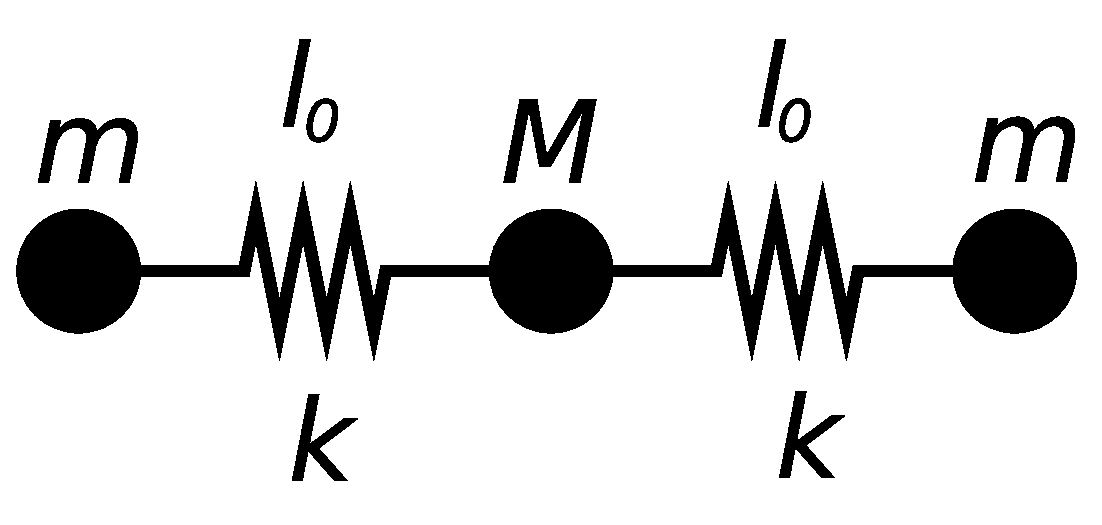
\includegraphics[width=\textwidth]{ej1-9}
\end{minipage}
\begin{enumerate}
	\item Encuentre las ecuaciones de movimiento de cada masa. 
	\item Halle las frecuencias de los modos normales. 
	\item Dibuje las configuraciones de cada modo. 
\item Si el centro de masa de la molécula  se mueve con $v_o=cte$, halle la solución para $\psi_a(t)$, $\psi_b(t)$ y $\psi_c(t)$.
	\item Determine las condiciones iniciales para excitar sólo el modo más alto (mayor frecuencia).
\end{enumerate}



\item
\begin{minipage}[t][2.2cm]{0.5\textwidth}
Analice las oscilaciones transversales del problema anterior.
Para su mejor comprensión puede imaginarlo como el esquema de la figura, en el cual las masas de los extremos pueden subir/bajar pero solidarios a la barra enhebrada a los vástagos laterales. 
\end{minipage}
\begin{minipage}[c][0cm][t]{0.45\textwidth}
  \includegraphics[width=\textwidth]{moleculaT}
\end{minipage}
\begin{enumerate}
	\item Encuentre las ecuaciones de movimiento de las masas. ¿Qué diferencias hay entre la ecuación de movimiento para resortes \emph{slinky} y resortes con $l_0\ne 0$ en la aprox. de pequeñas oscilaciones?
	\item Halle las frecuencias de los modos normales.
	\item Dibuje la configuración correspondiente a cada modo normal.
Determine los desplazamientos de cada masa como función del tiempo (solución más general posible para cada masa).
	\item ¿Qué condiciones iniciales que permiten excitar sólo el segundo modo?
	\item Si se fuerza la masa del centro con frecuencias incrementalmente mayores, ¿qué modos se van observando?
	\item ¿Cómo se modifican los resultados anteriores si el extremo de la derecha se fija a la pared como se indica en la figura a continuación?.
	\begin{figure}[h]
		\centering
		\includegraphics[clip,scale=0.5]{moleculaT_fijo_libre}
	\end{figure} 
\end{enumerate}



\item
\begin{minipage}[t][1.2cm]{0.6\textwidth}
(*) Considere el sistema de la figura, en la que los resortes verticales tienen longitud natural $l_0$ y constante $k_1$, y los horizontales $a_0= 0$ (``slinkies'') y $k_2$.
\end{minipage}
\begin{minipage}[c][2cm][t]{0.35\textwidth}
  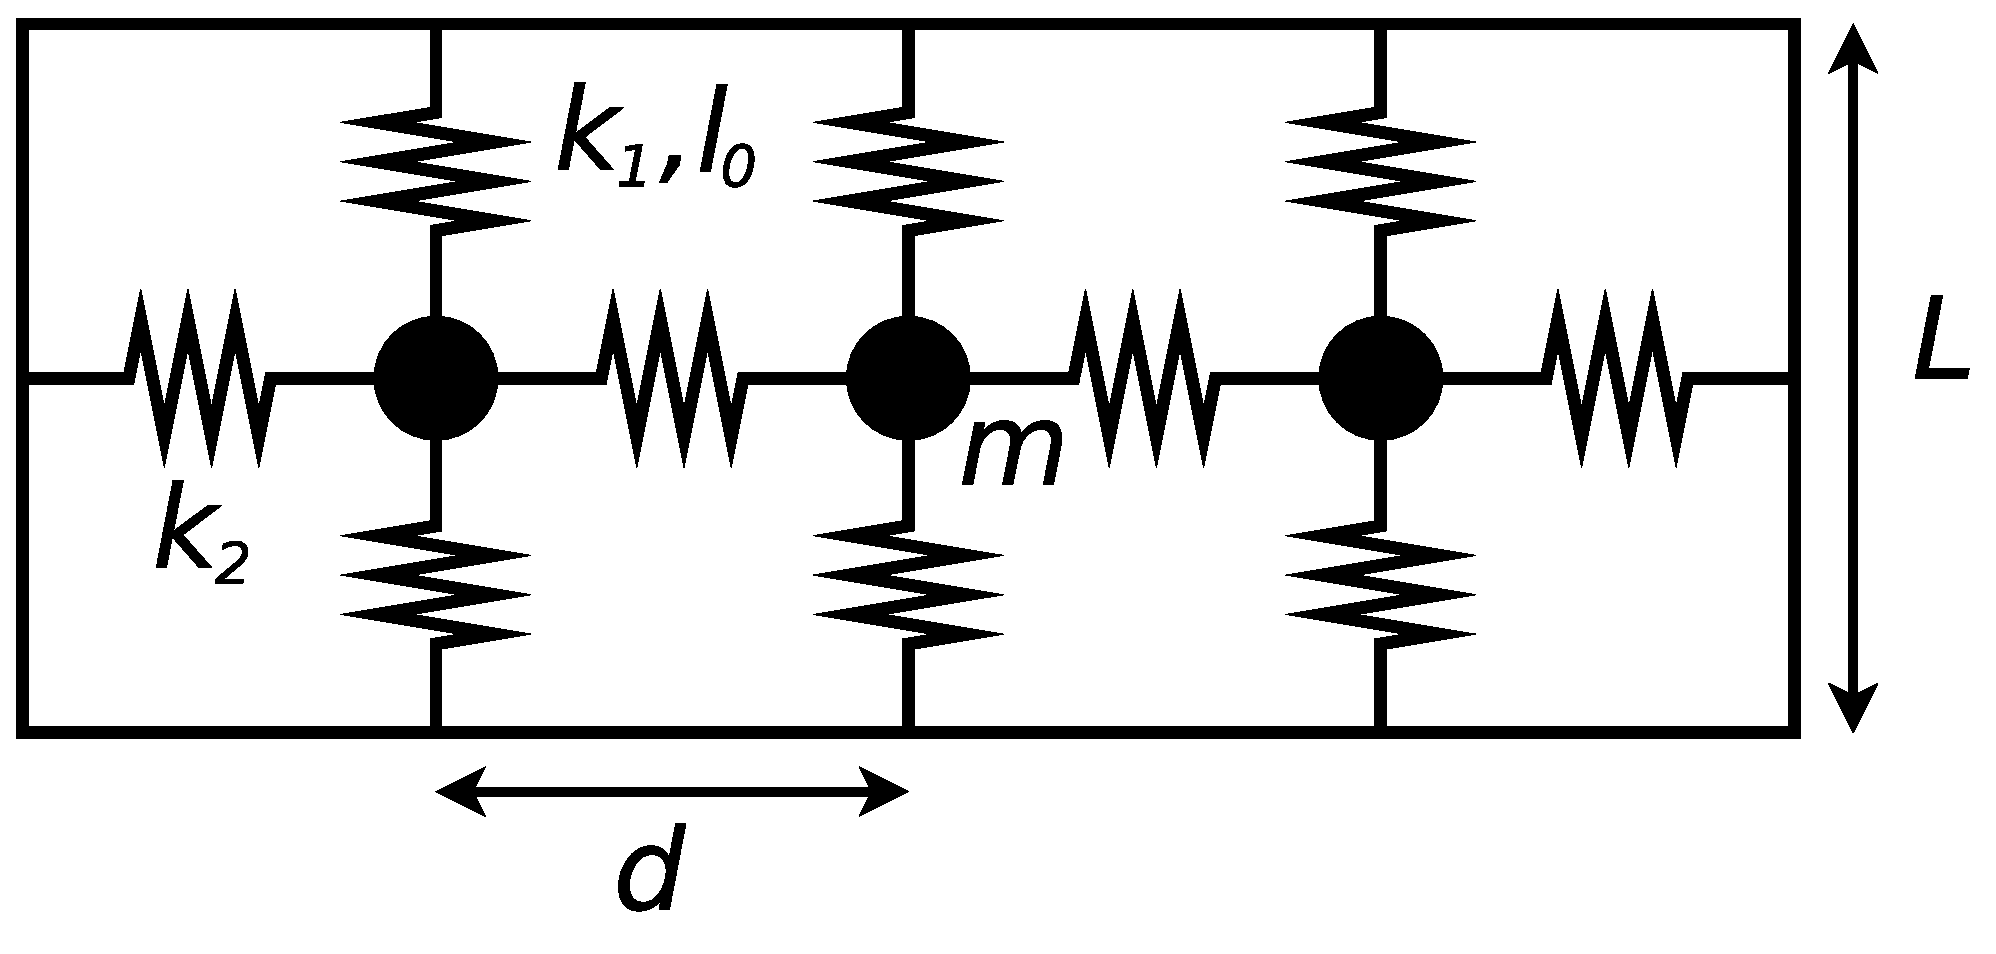
\includegraphics[width=\textwidth]{ej1-10}
\end{minipage}
\begin{enumerate}
  \item Calcule las frecuencias propias y los modos normales. 
  \item Considere que las condiciones iniciales son tales que el sistema oscila horizontalmente, estando su movimiento descripto por una superposición de los dos primeros modos.
  Halle la energía cinética de cada masa y la energía potencial del sistema, el promedio temporal de las mismas y la frecuencia de pulsación $\omega_{p}$.
\end{enumerate}



\end{enumerate}

\end{document}
